\documentclass{article}
\usepackage{graphicx}
\usepackage{amsmath}
\usepackage{amssymb}
\usepackage[italicdiff]{physics}
\usepackage{enumerate}
\usepackage{microtype}
\DisableLigatures{encoding= *, family=*}
\usepackage{titlesec}
\usepackage{xfrac}
\setcounter{secnumdepth}{4}
\usepackage{xcolor}
\usepackage[bookmarks=false]{hyperref}
\usepackage{mathtools}
\hypersetup{
    colorlinks=true,
    linkcolor=[RGB]{59 108 209},
    urlcolor=[RGB]{59 108 209}
}
\urlstyle{same}

\titleformat{\paragraph}
{\normalfont\normalsize\bfseries}{\theparagraph}{1em}{}
\titlespacing*{\paragraph}
{0pt}{3.25ex plus 1ex minus .2ex}{1.5ex plus .2ex}

\title{Inverse Trigonometric Functions}
\author{}
\date{}

\begin{document}
\maketitle

\section{Domain and Range of ITFs}

\subsection{Sine Inverse}

$f : [-1,1] \hspace{1mm} \xrightarrow{\hspace{4mm}} \left[-\dfrac{\pi}{2}, \dfrac{\pi}{2}\right], f(x)=\sin^{-1} x = \arcsin x$
\begin{center}
    
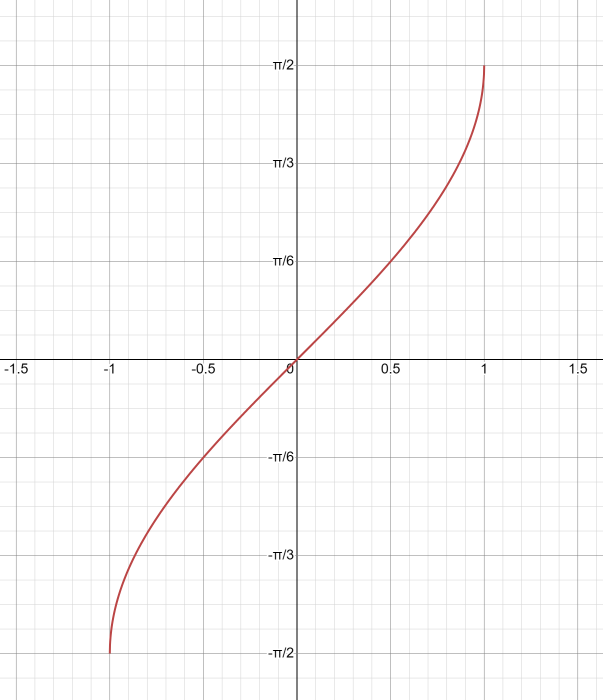
\includegraphics[scale=0.6]{graph_1.png}
\end{center}

\begin{itemize}
    \item The branch with range $\left[-\dfrac{\pi}{2}, \dfrac{\pi}{2}\right]$ is called \textbf{principal value branch}.
    \item The numerically least angle is called the \textbf{principal value branch}.
    \item $\sin^{-1} x$ is Bounded, Odd, Increasing, Aperiodic, Max (at $x=1$) $=\dfrac{\pi}{2}$, 
    \\Min (at $x=-1$) $=-\dfrac{\pi}{2}$ 
\end{itemize}
\subsection{Cosine Inverse}

$f : [-1,1] \hspace{1mm} \xrightarrow{\hspace{4mm}} \left[0,\pi\right], f(x)=\cos^{-1} x = \arccos x$

\begin{center}
    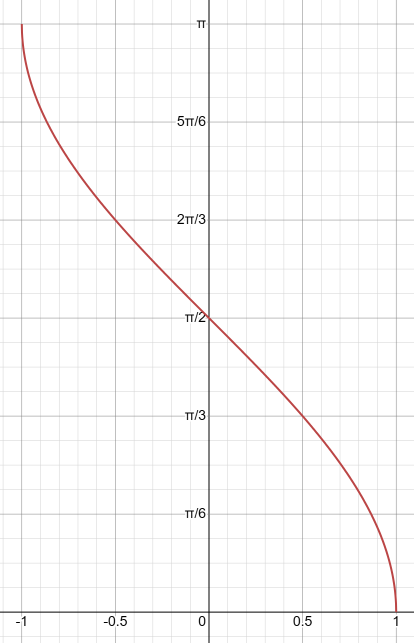
\includegraphics[scale=0.7]{graph_2.png}
\end{center}
\begin{itemize}
    \item Principal Value Branch for $\cos ^{-1} x$ is $\left[0,\pi\right]$
    \item $\cos^{-1}x$ is Bounded, Decreasing, Aperiodic, Max (at $x=-1$) $=\pi$, 
    \\Min (at $x=0$) $=0$
\end{itemize}
\newpage

\subsection{Tangent Inverse}

$f: \mathbb{R} \xrightarrow{\hspace{4mm}} \left[-\dfrac{\pi}{2},\dfrac{\pi}{2}\right], f(x)=\tan^{-1} x = \arctan x$
\begin{center}
    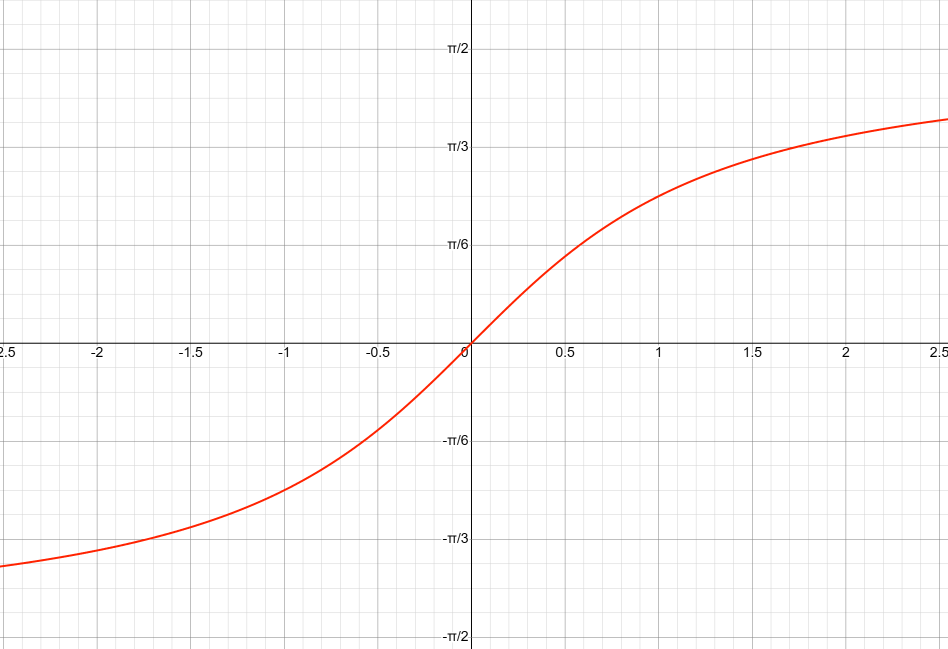
\includegraphics[scale=0.6]{graph_3.png}
\end{center}
\begin{itemize}
    \item Principal Value Branch for $\tan^{-1}x$ is $\left(-\dfrac{\pi}{2},\dfrac{\pi}{2}\right)$
    \item $\tan^{-1}x$ is Bounded, Odd, Increasing, Aperiodic, 
    \\Horizontal Asymptote $y=\pm \dfrac{\pi}{2}$
\end{itemize}
\newpage
\subsection{Cotangent Inverse}
$f:\mathbb{R} \xrightarrow{\hspace{4mm}} \left[0,\pi\right], f(x)=\cot^{-1}x=\arccot x$
\begin{center}
    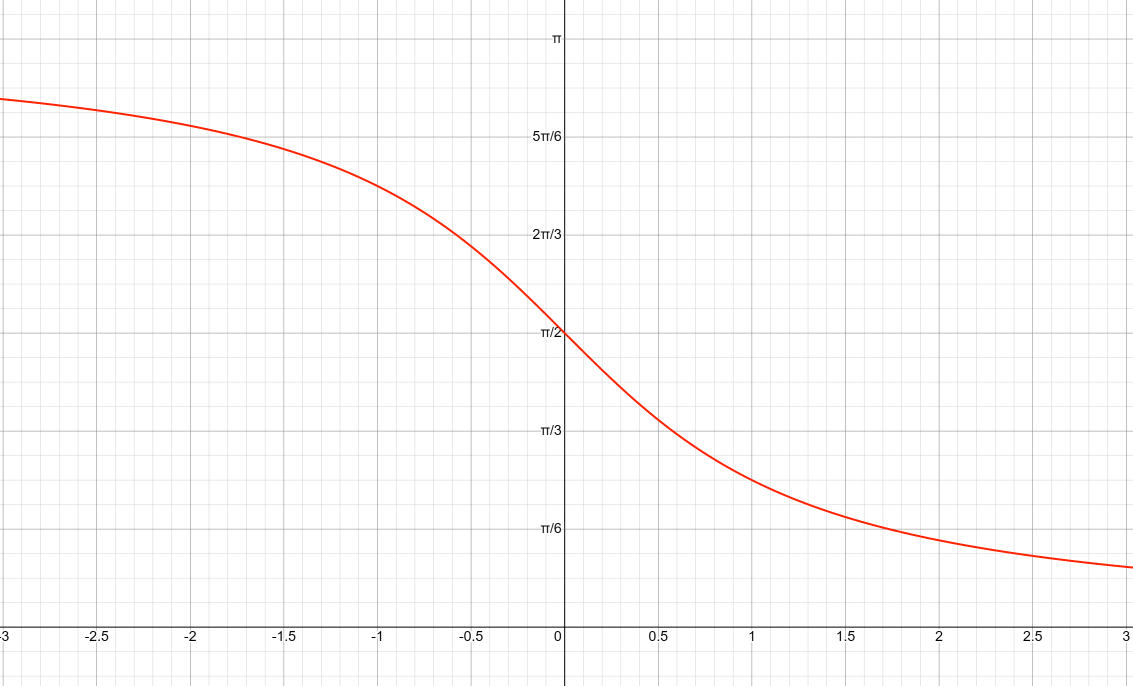
\includegraphics[scale=0.5]{graph_4.png}
\end{center}
\begin{itemize}
    \item Principal Value Branch for $\cot^{-1}x$ is $[0,\pi]$
    \item $\cot^{-1}x$ is Bounded, Decreasing, Aperiodic, 
    \\Horizontal Asymptote $y=0, y=\pi$
\end{itemize}
\newpage

\subsection{Secant Inverse}
$f: \mathbb{R}-(-1,1) \xrightarrow{\hspace{4mm}} \left[0,\pi\right]-\left\{\dfrac{\pi}{2}\right\}, f(x)=\sec^{-1}x=\arcsec x$
\begin{center}
    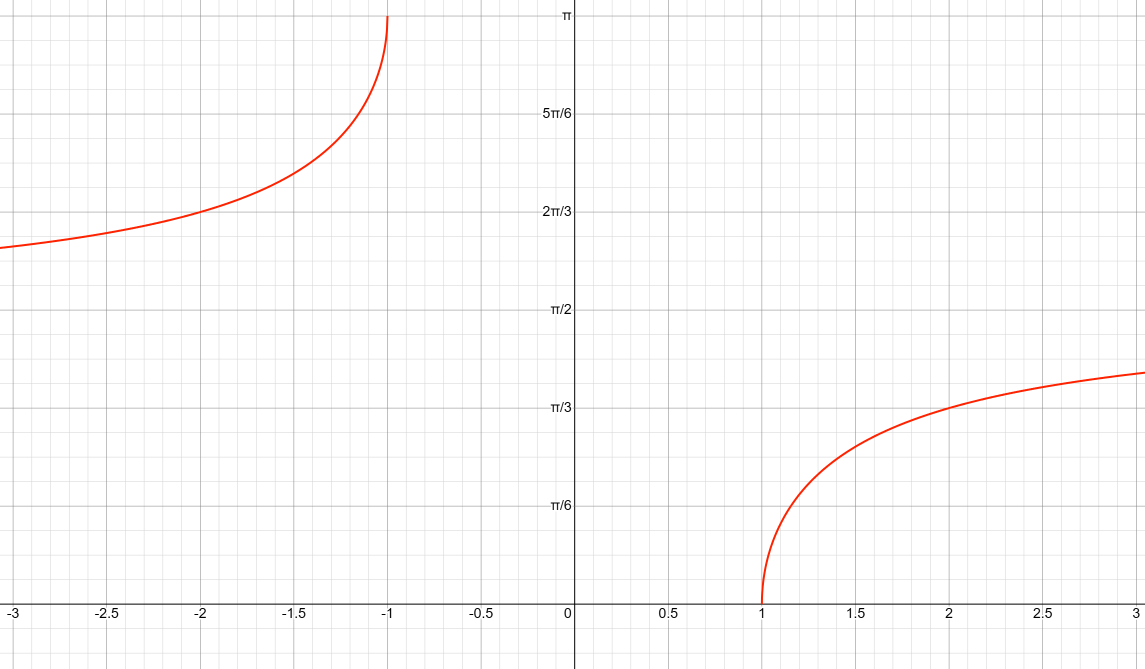
\includegraphics[scale=0.5]{graph_5.png}
\end{center}
\begin{itemize}
    \item Principal Value Branch for $\sec^{-1}x$ is $\left[0,\pi\right]-\left\{\dfrac{\pi}{2}\right\}$
    \item $\sec^{-1}x$ is Bounded, Increasing, Aperiodic, Max (at $x=-1$) $=\pi$, 
    \\Min (at $x=1$) $=0$, Horizontal Asymptote $y=\dfrac{\pi}{2}$
\end{itemize}
\newpage

\subsection{Cosecant Inverse}
$f:\mathbb{R}-(-1,1) \xrightarrow{\hspace{4mm}} \left[-\dfrac{\pi}{2},\dfrac{\pi}{2}\right]-\left\{0\right\}, f(x)=\csc^{-1}x=\arccsc x$

\begin{center}
    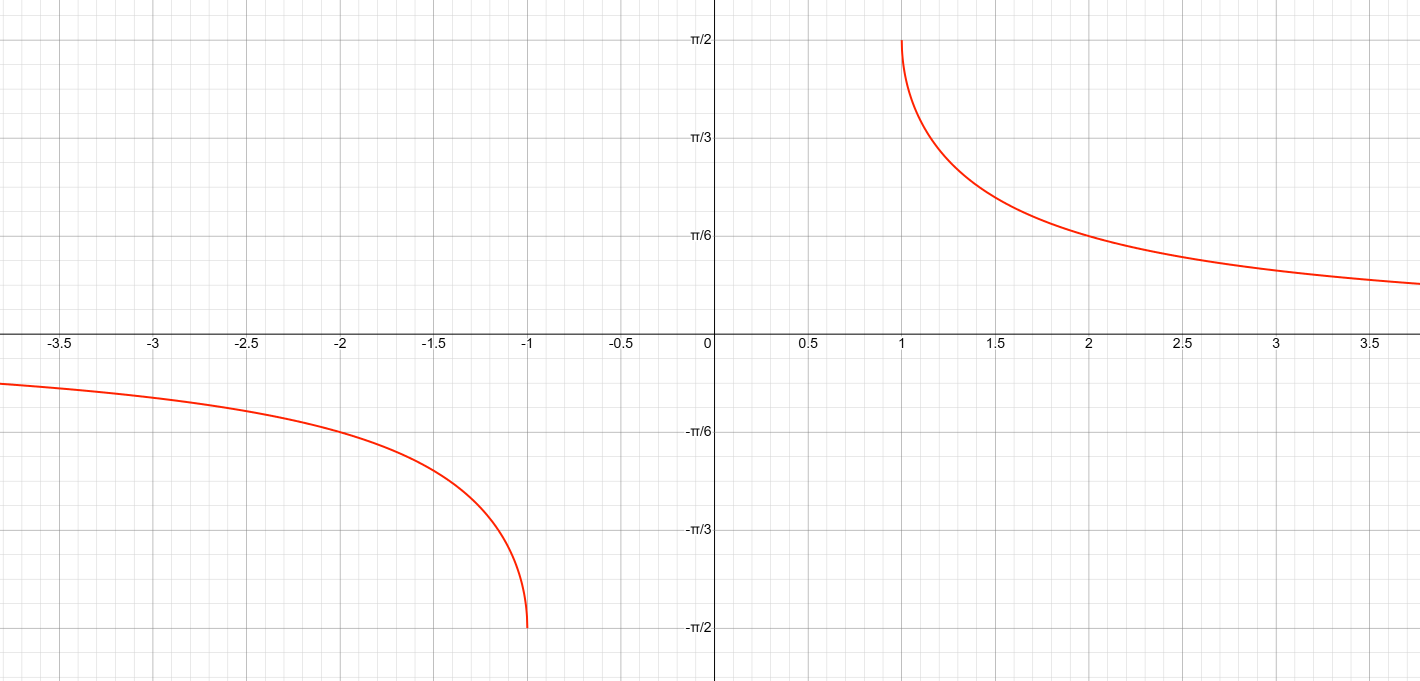
\includegraphics[scale=0.4]{graph_6.png}
\end{center}
\begin{itemize}
    \item Principal Value Branch for $\csc^{-1} x$ is $(0,\pi)$
    \item $\csc^{-1}x$ is Bounded, Odd, Decreasing, Aperiodic, Max (at $x=1$) $=\dfrac{\pi}{2}$, 
    \\Min (at $x=-1$) $=-\dfrac{\pi}{2}$, Horizontal Asymptote $y=0$
\end{itemize}
\section{Properties of ITFs}
\subsection{Inverse Composition Property}
\begin{enumerate}[i.]
    \item $\sin^{-1}(\sin x)=x \hfill \forall \hspace{2mm} x \in \left[\dfrac{-\pi}{2},\dfrac{\pi}{2}\right]$
    \item $\cos^{-1}(\cos x)=x \hfill \forall \hspace{2mm} x \in \left[0,\pi\right]$
    \item $\tan^{-1}(\tan x)=x \hfill \forall \hspace{2mm} x \in \left(-\dfrac{\pi}{2},\dfrac{\pi}{2}\right)$
    \item $\csc^{-1}(\csc x)=x \hfill \forall \hspace{2mm} x \in \left(-\dfrac{\pi}{2},\dfrac{\pi}{2}\right)-\left\{0\right\}$
    \item $\sec^{-1}(\sec x)=x \hfill \forall \hspace{2mm} x \in \left[0,\pi\right]-\left\{\dfrac{\pi}{2}\right\}$
    \item $\cot^{-1}(\cot x)=x \hfill \forall \hspace{2mm} x \in (0,\pi)$
\end{enumerate}

\subsection{Negative Argument Property}
\begin{enumerate}[i.]
    \item $\sin^{-1}(-x)=-\sin^{-1}x$
    \item $\tan^{-1}(-x)=-\tan^{-1}x$ 
    \item $\csc^{-1}(-x)=-\csc^{-1}x$
    \item $\cos^{-1}(-x)=\pi - \cos^{-1}x$
    \item $\cot^{-1}(-x)=\pi - \cot^{-1}x$
    \item $\sec^{-1}(-x)=\pi - \sec^{-1}x$
\end{enumerate}

\subsection{Trig. Composition Property}
\begin{enumerate}[i.]
    \item $\sin(\sin^{-1}x)=x \hfill \forall \hspace{2mm} x \in [-1,1]$
    \item $\cos(\cos^{-1}x)=x \hfill \forall \hspace{2mm} x \in [-1,1]$
    \item $\tan(\tan^{-1}x)=x \hfill \forall \hspace{2mm} x \in \mathbb{R}$
    \item $\csc(\csc^{-1}x)=x \hfill \forall \hspace{2mm} x \in \mathbb{R}-(-1,1)$
    \item $\sec(\sec^{-1}x)=x \hfill \forall \hspace{2mm} x \in \mathbb{R}-(-1,1)$
    \item $\cot(\cot^{-1}x)=x \hfill \forall \hspace{2mm} x \in \mathbb{R}$
\end{enumerate}

\subsection{Argument Reciprocal Property}
\begin{enumerate}[i.]
    \item $\csc^{-1}x=\sin^{-1}\left(\dfrac{1}{x}\right) \hfill \forall \hspace{2mm} x \in \mathbb{R}-(-1,1)$
    \item $\sin^{-1}x=\csc^{-1}\left(\dfrac{1}{x}\right) \hfill \forall \hspace{2mm} x \in [-1,1]-\left\{0\right\}$
    \item $\sec^{-1}x=\cos^{-1}\left(\dfrac{1}{x}\right) \hfill \forall \hspace{2mm} x \in \mathbb{R}-(-1,1)$
    \item $\cos^{-1}x=\sec^{-1}\left(\dfrac{1}{x}\right) \hfill \forall \hspace{2mm} x \in [-1,1]-\left\{0\right\}$
    \item $\cot^{-1}x=\begin{cases}
        \tan^{-1}\left(\dfrac{1}{x}\right) & x > 0 \\
        \pi + \tan^{-1}\left(\dfrac{1}{x}\right) & x<0
    \end{cases}$
    \item $\tan^{-1}x=\begin{cases}
        \cot^{-1}\left(\dfrac{1}{x}\right) & x>0 \\
        -\pi + \cot^{-1}\left(\dfrac{1}{x}\right) & x<0
    \end{cases}$
\end{enumerate}

\subsection{Complementary Angle Property}
\begin{enumerate}[i.]
    \item $\sin^{-1}x+\cos^{-1}x=\dfrac{\pi}{2} \hfill \forall \hspace{2mm} x \in [-1,1] $
    \item $\tan^{-1}x+\cot^{-1}x=\dfrac{\pi}{2} \hfill \forall \hspace{2mm} x \in \mathbb{R} $
    \item $\sec^{-1}x+\csc^{-1}x=\dfrac{\pi}{2} \hfill \forall \hspace{2mm} x \in \mathbb{R}-(-1,1) $
\end{enumerate}

\subsection{Sum Property}
\begin{enumerate}[i.]
    \item $\tan^{-1}x+\tan^{-1}y=\begin{cases}
        \tan^{-1}\left(\dfrac{x+y}{1-xy}\right) & xy<1 \\
        \pi + \tan^{-1}\left(\dfrac{x+y}{1-xy}\right) & x>0, y>0, xy>1 \\
        -\pi + \tan^{-1}\left(\dfrac{x+y}{1-xy}\right) & x<0, y<0, xy>1
    \end{cases}$
    \item $\tan^{-1}x-\tan^{-1}y=\begin{cases}
        \tan^{-1}\left(\dfrac{x-y}{1+xy}\right) & xy>-1 \\
        \pi +\tan^{-1}\left(\dfrac{x-y}{1+xy}\right) & x>0, y<0, xy<-1 \\
        -\pi +\tan^{-1}\left(\dfrac{x-y}{1+xy}\right) & x<0, y>0, xy<-1
    \end{cases}$
    \item $\tan^{-1}x_{1}+\tan^{-1}x_{2}+ \ldots + \tan^{-1}x_{n}=\tan^{-1}\left(\dfrac{S_{1}-S_{3}+S_{5}- \ldots}{1-S_{2}+S_{4}-S_{6}+\ldots}\right) \hfill \\ \hphantom{2cm} \hspace{5cm} \forall \hspace{2mm} x_{i} \in \mathbb{R}, i \in \mathbb{N}$
    \item $\sin^{-1}x+\sin^{-1}y=\begin{cases}
        \sin^{-1}\left(x+\sqrt{1-y^2}+y\sqrt{1-x^2}\right) & x\ge -1, y \le 1, x^2+y^2 \le 1\\
        \pi - \sin^{-1}\left(x\sqrt{1-y}+y\sqrt{1-x^2}\right) & x > 0, y \le 1, x^2+y^2>1 \\
        -\pi - \sin^{-1}\left(x\sqrt{1-y}+y\sqrt{1-x^2}\right) & x \ge -1, y < 0, x^2+y^2 >1
    \end{cases}$
    \item 
\end{enumerate}
\end{document}